\subsection{Zeri di funzione}

\subsubsection{Grafici di funzione}

In MATLAB una funzione $f\left(x\right)$ viene memorizzata come un vettore. In particolare, il vettore $y$ ottenuto valutando $f$ nel vettore delle ascisse $x$. Per cui la rappresentazione della funzione $f\left(x\right)$ è di fatto la rappresentazione del vettore $y$ contro il vettore $x$.

\highspace
Per introdurre i concetti di funzione e grafici di funzione, si presentano qua di seguito alcuni esempi di caso d'uso.

\highspace
\example{\emph{Definire le seguenti variabili:
\begin{itemize}
    \item $x$: vettore di estremi $0$ e $10$ con passo $0.1$
    \item $y = e^{x} + 1$
\end{itemize}}}

\noindent
Il vettore delle ascisse $x$ può essere costruito banalmente con il seguente costrutto:
\begin{lstlisting}[language=MATLAB]
x = [0 : 0.1 : 10];\end{lstlisting}
Per quanto riguarda la \textbf{funzione}, si utilizza la keyword \texttt{\@} per indicare che $f$ ha come input un valore (\texttt{x}) e rappresenta la funzione \texttt{exp(x)+1}. In questo caso, la funzione si dice anonima. Per dichiarare funzioni esplicite, si rimanda alla \href{https://it.mathworks.com/help/releases/R2024a/matlab/ref/function_handle.html}{documentazione ufficiale}.
\begin{lstlisting}[language=MATLAB]
f = @(x) exp(x) + 1\end{lstlisting}
Una volta definita una \textbf{funzione}, per \textbf{valutarla in uno o più punti}, si utilizzerà banalmente la sintassi matematica:
\begin{lstlisting}[language=MATLAB]
f(2)

ans =

    8.3891

f(0:3)

ans =

    2.0000    3.7183    8.3891   21.0855\end{lstlisting}
Da notare che se l'argomento è un vettore, allora il risultato sarà un vettore della medesima lunghezza del vettore dato in input.

\newpage

\noindent
\example{\emph{Utilizzando le variabili precedentemente definite, disegnare il grafico della funzione $y = e^{x} + 1$ nell'intervallo $\left[0, 10\right]$.}}

\highspace
Per disegnare il grafico si utilizza il comando \texttt{plot}. Di default questa funzione disegna i valori in un piano cartesiano usando segmenti rettilinei (retta spezzata):
\begin{lstlisting}[language=MATLAB]
y = f(x);
plot(x, y)\end{lstlisting}
\begin{figure}[!htp]
    \centering
    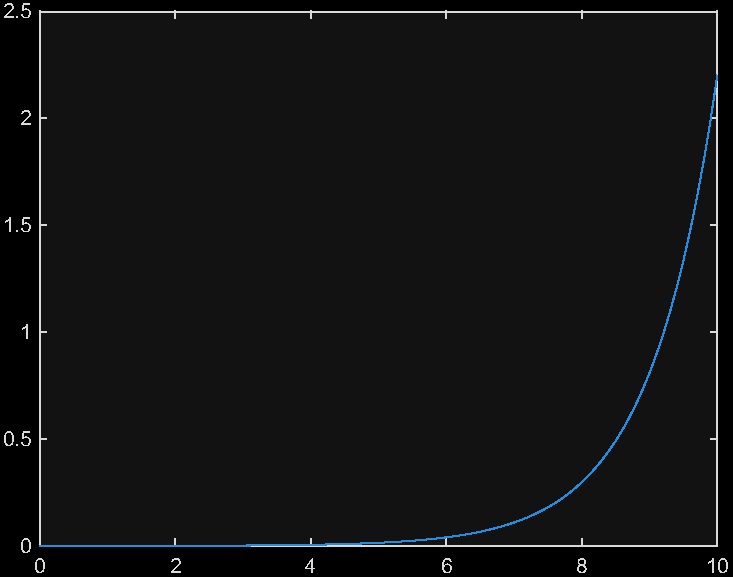
\includegraphics[width=.6\textwidth]{img/grafici-di-funzione-1.pdf}
\end{figure}

\noindent
Per evitare che MATLAB sovrascriva la figura nella finestra aperta, è possibile numerarle usando la funzione \texttt{figure} (e.g. \texttt{figure(1); plot(x,y); figure(2); plot(0:3, 0:3)}).

\highspace
La funzione \texttt{plot} accetta determinati valori per modificare il grafico finale. Nella \href{https://it.mathworks.com/help/releases/R2024a/matlab/ref/plot.html}{documentazione ufficiale} è possibile trovare l'intera lista e alcuni esempi. Scrivendo \texttt{plot(x, f(x), 'linewidth', 2)}, il parametro \texttt{'linewidth'} consente di definire lo spessore delle curve. Il valore che viene specificato in questo caso è \texttt{2} e il risultato:
\begin{figure}[!htp]
    \centering
    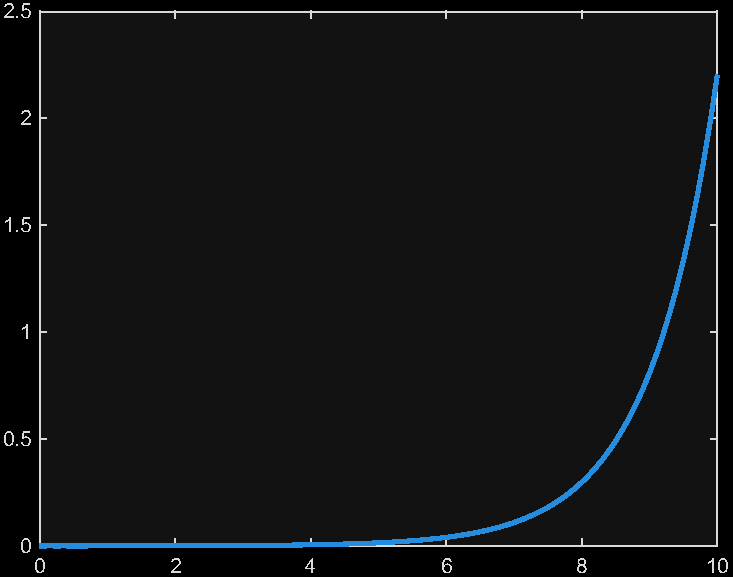
\includegraphics[width=.6\textwidth]{img/grafici-di-funzione-2.pdf}
\end{figure}

\newpage

\noindent
Usando il comando \texttt{hold on} per fare un confronto tra i vari grafici e invocando di nuovo la funzione \texttt{plot} ma con parametri differenti, si ottiene:
\begin{lstlisting}[language=MATLAB]
figure(1)
plot(x, f(x), 'linewidth', 2)
hold on
plot(x, -f(x), 'r', 'linewidth', 2)\end{lstlisting}

\begin{figure}[!htp]
    \centering
    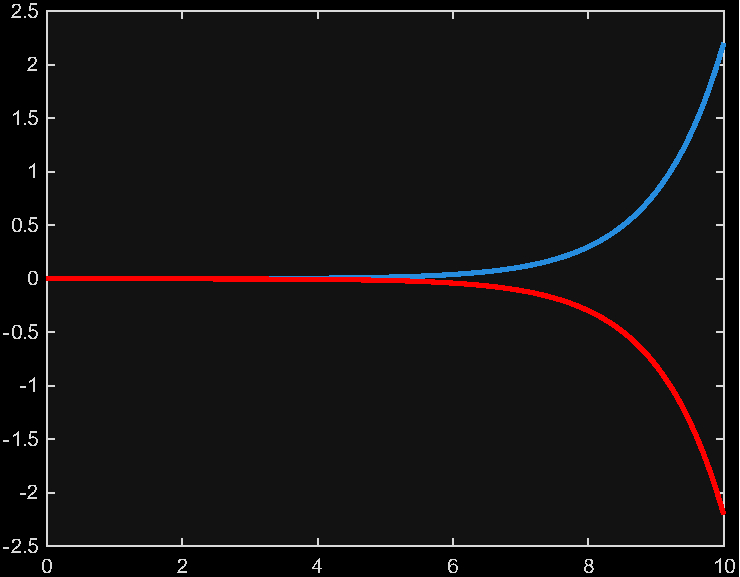
\includegraphics[width=.6\textwidth]{img/grafici-di-funzione-3.pdf}
\end{figure}

\noindent
\example{\emph{Disegnare il grafico in scala semi-logaritmica (logaritmica solo per le ordinate) della funzione $y = e^{x}$ nell'intervallo $\left[0, 10\right]$. È possibile prevedere come sarà il grafico in scala semi-logaritmica della funzione $y=e^{2x}$? Verificare la risposta tracciando sulla medesima finestra le due funzioni utilizzando colori diversi per i due grafici.}}

\highspace
Per disegnare il grafico in scala semi-logaritmica (logaritmica sulle ordinate) si utilizza il comando \texttt{semilogy} e si aggiunge anche la griglia:
\begin{lstlisting}[language=MATLAB]
semilogy(x, exp(x), 'linewidth', 2)
grid on\end{lstlisting}
\begin{figure}[!htp]
    \centering
    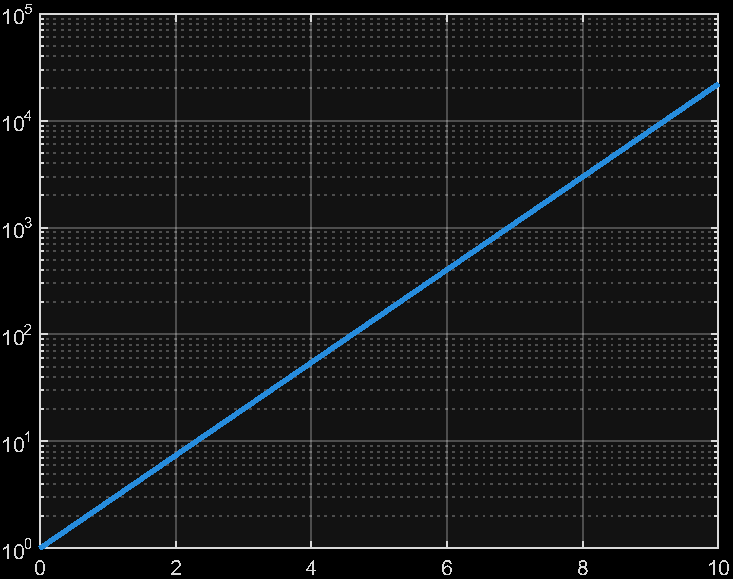
\includegraphics[width=.6\textwidth]{img/grafici-di-funzione-4.pdf}
    \caption*{È una retta poiché $\log_{10}\left(y\right) = \log_{10}\left(e^{x}\right) = x\log_{10}\left(e\right)$.}
\end{figure}

\begin{itemize}
    \item Il comando \texttt{semilogy} è l'equivalente di \texttt{plot} ma traccia un \textbf{grafico con l'asse delle ordinate in scala logaritmica}.

    \item Il comando \texttt{semilogx} traccia un \textbf{grafico con l'asse delle ascisse logaritmico}.
    
    \item Il comando \texttt{loglog} traccia un grafico in cui entrambi gli assi sono in scala logaritmica.
\end{itemize}
Passando alla risoluzione dell'esercizio, dato che $\log_{10}\left(e^{2x}\right) = 2x\log_{10}\left(e\right)$, disegnando in scala semi-logaritmica la funzione $y = e^{2x}$, si otterrà una retta con pendenza doppia rispetto alla retta precedentemente disegnata.
\begin{lstlisting}[language=MATLAB]
hold on
semilogy(x, exp(2 * x), 'r', 'linewidth', 2)
% oppure in un solo comando senza usare hold on
% semilogy(x, exp(x), 'b', x, exp(2*x), 'r', 'linewidth', 2)
title('Grafico di exp(x) e di exp(2x)')
xlabel('Scala lineare')
ylabel('Scala logaritmica')
grid on
legend('exp(x)', 'exp(2*x)', 'Location', 'NorthWest')\end{lstlisting}
\begin{figure}[!htp]
    \centering
    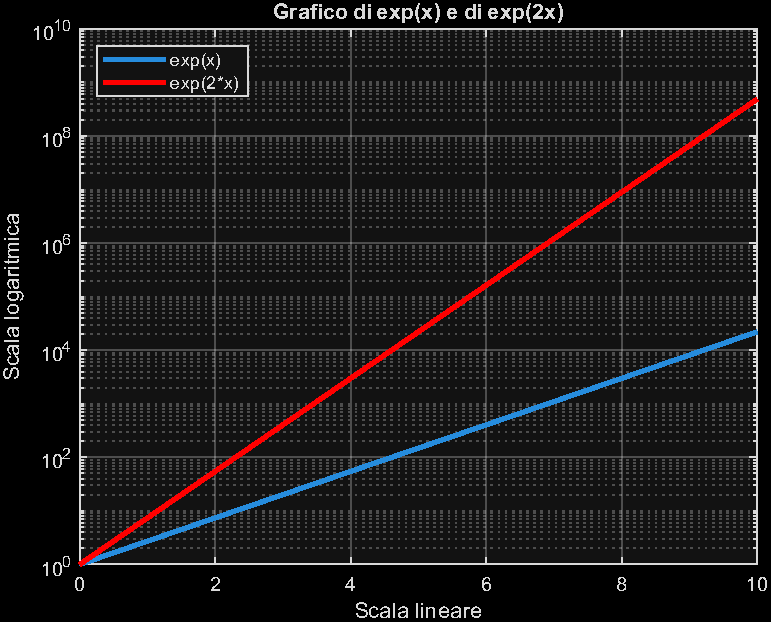
\includegraphics[width=.7\textwidth]{img/grafici-di-funzione-5.pdf}
\end{figure}

\noindent
Il comando \texttt{legend} attribuisce alle curve disegnate da \texttt{plot} le stringhe di testo che gli vengono passate. Attenzione che alcune stringhe, come \texttt{'Location'} e \texttt{'NorthWest'}, vengono interpretate dalla funzione come comandi veri e propri. In questo caso si chiede di inserire una legenda in alto a sinistra.